\documentclass{report}
\usepackage{pgf,tikz,pgfplots}
\pgfplotsset{compat=1.15}
\usepackage{mathrsfs}
\usetikzlibrary{arrows}
\usepackage{float}

\title{Solutions for Calculus Vol 1: One variable calculus, with an introduction to Linear Algebra (2nd Edition) by Tom M. Apostol}
\author{Michael Rocke}

\begin{document}
\maketitle

\tableofcontents

\section{Introduction}

\subsection{1.4 Exercises}

\subsubsection{1}

\begin{figure}[H]

		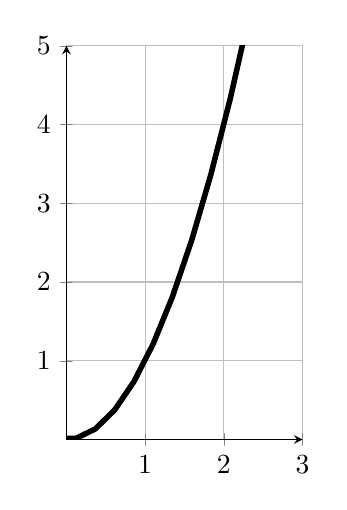
\begin{tikzpicture}[line cap=round,line join=round,>=triangle 45,x=1cm,y=1cm]
		\begin{axis}[
		x=1cm,y=1cm,
		axis lines=middle,
		ymajorgrids=true,
		xmajorgrids=true,
		xmin=0,
		xmax=3,
		ymin=0,
		ymax=5,
		xtick={-12,-11,...,4},
		ytick={-9,-8,...,9},]
		\clip(-12.92,-9.52) rectangle (4.92,9.52);
		\draw [samples=50,rotate around={0:(0,0)},xshift=0cm,yshift=0cm,line width=2pt,domain=-6:6)] plot (\x,{(\x)^2/2/0.5});
		\begin{scriptsize}
		\draw[color=black] (-1.7,1.03) node {$y = x^2$};
		\end{scriptsize}
		\end{axis}
		\end{tikzpicture}
		
		Figure 1.3: $y=x^2$
\end{figure}

a) Modify the region in Figure 1.3 by assuming that the ordinate at each $x$ is $2x^2$ instead of $x^2$. 

Draw the new figure. 

\begin{figure} [H]
	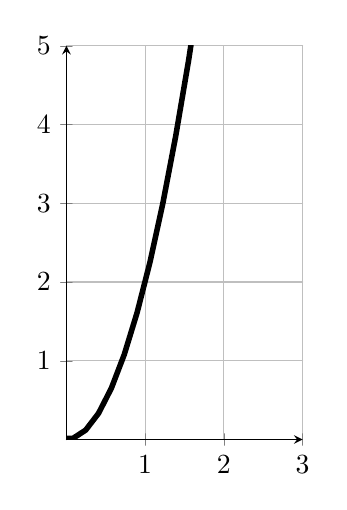
\begin{tikzpicture}[line cap=round,line join=round,>=triangle 45,x=1cm,y=1cm]
	\begin{axis}[
	x=1cm,y=1cm,
	axis lines=middle,
	ymajorgrids=true,
	xmajorgrids=true,
	xmin=0,
	xmax=3,
	ymin=0,
	ymax=5,
	xtick={-12,-11,...,4},
	ytick={-9,-8,...,9},]
	\clip(-12.92,-9.52) rectangle (4.92,9.52);
	\draw [samples=50,rotate around={0:(0,0)},xshift=0cm,yshift=0cm,line width=2pt,domain=-4:4)] plot (\x,{(\x)^2/2/0.25});
	\begin{scriptsize}
	\draw[color=black] (-1.12,0.53) node {$y = 2x^2$};
	\end{scriptsize}
	\end{axis}
	\end{tikzpicture}
	
	$y = 2x^2$
\end{figure}

Check through the principal steps in the forgoing section and find what effect this has on the calculation of the area. Do the same if the ordfinate at each $x$

b) $3x^2$

\begin{figure}[H]

		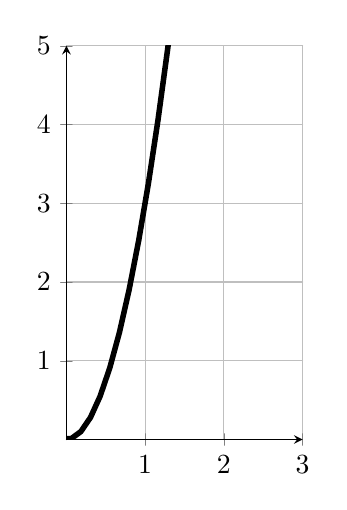
\begin{tikzpicture}[line cap=round,line join=round,>=triangle 45,x=1cm,y=1cm]
		\begin{axis}[
		x=1cm,y=1cm,
		axis lines=middle,
		ymajorgrids=true,
		xmajorgrids=true,
		xmin=0,
		xmax=3,
		ymin=0,
		ymax=5,
		xtick={-12,-11,...,4},
		ytick={-9,-8,...,9},]
		\clip(-12.92,-9.52) rectangle (4.92,9.52);
		\draw [samples=50,rotate around={0:(0,0)},xshift=0cm,yshift=0cm,line width=2pt,domain=-3:3)] plot (\x,{(\x)^2/2/0.16666666666666666});
		\begin{scriptsize}
		\draw[color=black] (-0.96,0.37) node {$y = 3x^2$};
		\end{scriptsize}
		\end{axis}
		\end{tikzpicture}
		
		$y = 3x^2$
\end{figure}

c) $\frac{1}{4}x^2$

\begin{figure}[H]
	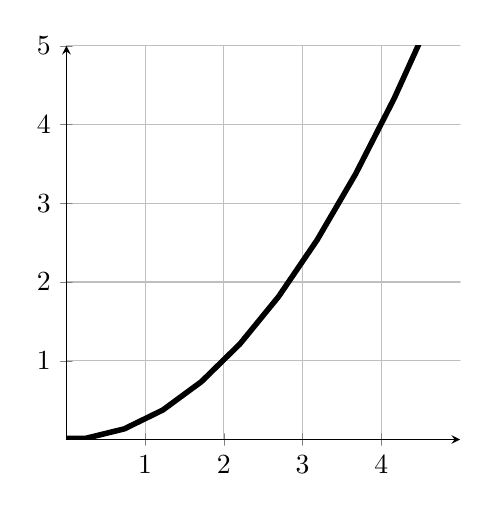
\begin{tikzpicture}[line cap=round,line join=round,>=triangle 45,x=1cm,y=1cm]
	\begin{axis}[
	x=1cm,y=1cm,
	axis lines=middle,
	ymajorgrids=true,
	xmajorgrids=true,
	xmin=0,
	xmax=5,
	ymin=0,
	ymax=5,
	xtick={-12,-11,...,4},
	ytick={-9,-8,...,9},]
	\clip(-12.92,-9.52) rectangle (4.92,9.52);
	\draw [samples=50,rotate around={0:(0,0)},xshift=0cm,yshift=0cm,line width=2pt,domain=-12:12)] plot (\x,{(\x)^2/2/2});
	\begin{scriptsize}
	\draw[color=black] (-4.38,4.03) node {$y = x^2 / 4$};
	\end{scriptsize}
	\end{axis}
	\end{tikzpicture}
	
	$y = \frac{1}{4} x^2$
\end{figure}

d) $2x^2 + 1$

e) $ax^2 + c$

\subsubsection{2}

Modify the region in Figure 1.3 by assuming that the ordinate at each $x$ is $x^3$ instead of $x^2$.

Draw the new figure.

a) Use a construction similar to that illustrated in Figure 1.5 and show that the outer and inner sums $S_n$ and $s_n$ are given by

\[
S_n = \frac{b^4}{n^4} (1^3 + 2^3 + ... + n^3), \; s_n = \frac{b^4}{n^4}[1^3 + 2^3 + ... + (n - 1)^3]
\]


b)
\end{document}